% Created 2017-03-28 Tue 08:00
\documentclass[10pt,t,a4paper]{beamer}
\usepackage[utf8]{inputenc}
\usepackage[T1]{fontenc}
\usepackage{fixltx2e}
\usepackage{graphicx}
\usepackage{longtable}
\usepackage{float}
\usepackage{wrapfig}
\usepackage{rotating}
\usepackage[normalem]{ulem}
\usepackage{amsmath}
\usepackage{textcomp}
\usepackage{marvosym}
\usepackage{wasysym}
\usepackage{amssymb}
\usepackage{hyperref}
\tolerance=1000
\usetheme{BTH_msv}
\author{Mikael Svahnberg\thanks{Mikael.Svahnberg@bth.se}}
\date{\today}
\title{Software Design\\\\Introduction}
\hypersetup{
  pdfkeywords={},
  pdfsubject={},
  pdfcreator={Emacs 25.1.1 (Org mode 8.2.10)}}
\begin{document}

\maketitle

\begin{frame}[label=sec-1]{About Me: Mikael Svahnberg}
\includegraphics[width=1.5cm]{/Users/msv/Documents/Personal/avartar.png}
\begin{itemize}
\item Associate Professor, PhD in Software Engineering
\item \url{mailto:Mikael.Svahnberg@bth.se}
\item \url{https://sites.google.com/site/mikaelsvahnberg/}
\item Interests:
\begin{itemize}
\item Software Architectures, Software Architecture Evaluation, Software Architecture Evolution, Requirements Engineering, Large Scale Requirements Engineering, Market-Driven Requirements Engineering, Software Product Lines, Software Reuse, Empirical Research Methodology, Software Engineering Decision Support, Static Code Analysis, Software Architecture Reconstruction
\end{itemize}
\end{itemize}
\end{frame}
\begin{frame}[label=sec-2]{Discuss: Course Charter: PA1415}
Efter genomförd kurs skall studenten:
\begin{itemize}
\item på en grundläggande nivå i grupp kunna ta fram krav på en programvara och uttrycka dem i en kravspecifikation
\item i grupp producera en översiktlig utvecklingsprojektplan baserat på en kravspecifikation
\item i grupp kunna skapa en detaljerad objektorienterad design för ett mjukvaruprogram
\item i grupp kunna implementera ett mjukvaruprogram inom rimlig tid, baserat på en kravspecifikation och en objektorienterad design
\item på en grundläggande nivå i grupp kunna planera och genomföra testning av producerad programvara, baserat på en kravspecifikation
\item skapa och analysera objektorienterade artefakter uttryckta i UML
\item kunna motivera och använda designmönster i utvecklingen av mjukvarusystem
\end{itemize}
\end{frame}
\begin{frame}[shrink=15,label=sec-3]{Discuss: Course Charter: PA1435}

\alert{Kunskap och förståelse} Efter genomförd kurs ska studenten:
\begin{itemize}
\item kunna visa förståelse för grundläggande principer i objektorienterad programvaruutveckling.
\item kunna visa förståelse för UML som modelleringsspråk.
\item kunna visa kunskap om grundläggande designprinciper.
\item kunna visa kunskap om grundläggande designmönster.
\end{itemize}

\alert{Färdigheter och förmåga} Efter genomförd kurs ska studenten:
\begin{itemize}
\item kunna uttrycka strukturen och beteendet hos ett system i termer av objektorienterade koncept.
\item kunna korrekt använda UML för att uttrycka struktur och beteende hos ett system.
\item kunna korrekt transformera en objektorienterad design till källkod.
\item kunna tillämpa designprinciper och designmönster i allmänhet och inom en särskild domän.
\end{itemize}

\alert{Värderingsförmåga och förhållningssätt} Efter genomförd kurs ska studenten:
\begin{itemize}
\item kunna analysera källkod för eventuella förbättringar.
\item kunna analysera och kritiskt diskutera en design för eventuella förbättringar.
\end{itemize}
\end{frame}
\begin{frame}[shrink=15,label=sec-4]{Discuss: Course Charter: PA1443}

\alert{Kunskap och förståelse} Efter genomförd kurs ska studenten:
\begin{itemize}
\item kunna visa förståelse för grundläggande principer i objektorienterad programvaruutveckling.
\item kunna visa kunskap om grundläggande designprinciper.
\item kunna visa kunskap om grundläggande designmönster.
\item kunna visa kunskap om grundläggande mjukvaruarkitekturstilar
\end{itemize}

\alert{Färdigheter och förmåga} Efter genomförd kurs ska studenten:
\begin{itemize}
\item kunna uttrycka strukturen och beteendet hos ett system i termer av objektorienterade koncept.
\item kunna tillämpa grundläggande designmönster i en objektorienterad design.
\item kunna skapa en objektorienterad design för ett system enligt goda objektorienterade designprinciper
\item kunna tillämpa grundläggande arkitekturstilar för ett mjukvarusystem
\item kunna resonera om de kvalitetsegenskaper ett system med en viss arkitekturstil har eller bör ha
\item kunna resonera om och skapa en grundläggande testplan för ett objektorienterat system
\end{itemize}

\alert{Värderingsförmåga och förhållningssätt} Efter genomförd kurs ska studenten:
\begin{itemize}
\item kunna analysera och kritiskt diskutera en design för eventuella förbättringar.
\end{itemize}
\end{frame}
\begin{frame}[label=sec-5]{Course Structure}
\begin{itemize}
\item \url{https://mickesv.github.io/OODesign/}

\item Sprints
\item Lectures
\begin{itemize}
\item Video Lectures
\item Classroom Lectures
\end{itemize}
\item Seminars
\item Assignments (Release Sprints)
\end{itemize}

See \href{https://mickesv.github.io/OODesign/Sprint0-course-intro.html}{Sprint 0: Course Introduction} homepage on It's for deadlines etc.        
\end{frame}
\begin{frame}[shrink=15,label=sec-6]{Literature}

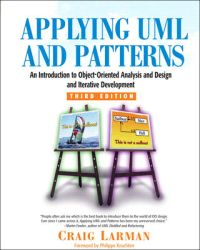
\includegraphics[width=1.5cm]{./ILarman.jpg}
\begin{itemize}
\item C. Larman, \emph{Applying UML and Patterns}, Prentice Hall, 3rd Edition
\item Also available as a softcover edition from 2015
\end{itemize}

\only<2>{
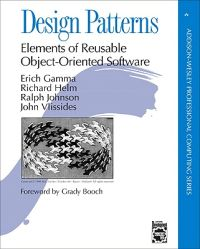
\includegraphics[height=1.5cm]{./IGamma.jpg}
\begin{itemize}
\item Gamma, Helm, Johnson, Vlissides, \emph{Design Patterns, Elements of Reusable Object-Oriented Software}, Addison-Wesley Professional
\end{itemize}
}
\end{frame}
\begin{frame}[label=sec-7]{Tools}
Any UML Tool will work, except pen and paper.

\begin{itemize}
\item \url{http://staruml.io/}
\item \url{https://www.visual-paradigm.com/}
\item \url{http://www.eclipse.org/papyrus/}
\item \url{http://argouml.tigris.org/}
\item \url{https://marketplace.eclipse.org/content/uml-designer}
\item \url{http://plantuml.com/}
\item \ldots{}
\end{itemize}
\end{frame}
\begin{frame}[label=sec-8]{Discuss: Why Bother About Modelling}
T. Gorschek, E. Tempero, L. Angelis, \emph{On the use of software design models in software development practice: An empirical investigation}, in Journal of Systems and Software 95(2014):176--193.

\begin{itemize}
\item TL;DR: Nearly 4000 industry practitioners were asked ``Do you model?''. Answers ranged from ``no'' to ``hell no!''.
\end{itemize}
\only<2>{
\begin{itemize}
\item \ldots{} \alert{There is, of course, more to this story.}
\end{itemize}
} \vspace{0.25cm}
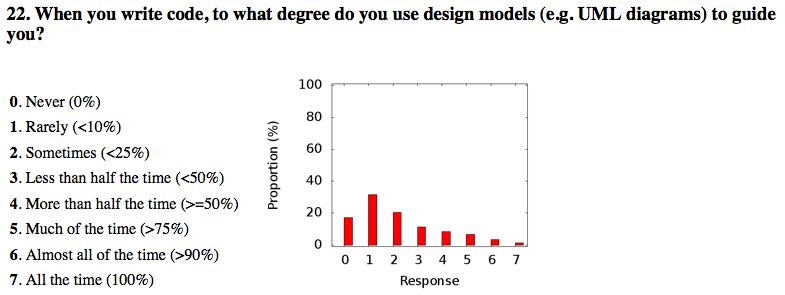
\includegraphics[width=9cm]{./ISurveyModelling.png}
\end{frame}
\begin{frame}[label=sec-9]{Why Bother About Modelling}
\begin{itemize}
\item In the freetext answers a different story emerges:
\begin{itemize}
\item They do use sketches, informal models, casual diagrams, etc, but not formal UML.
\end{itemize}
\item Common explanations:
\begin{itemize}
\item ``Only for very complex designs, sometimes''
\item ``Only use initially then start coding (diagrams not kept/updated)"
\item ``Enables visualisation of the big picture/high level''
\item ``Other types of models but not UML''
\item ``Use models to communicate and coordinate with other developers''
\end{itemize}
\item $\sum$ Models are not used as researchers expect. Instead they are used for \alert{conceptual analysis and exploration, problem solving, visualisation, and communication.}
\end{itemize}
\end{frame}
\begin{frame}[label=sec-10]{So, why bother?}
\begin{itemize}
\item conceptual analysis and exploration
\item problem solving
\item visualisation
\item communication
\end{itemize}

Also:
\begin{itemize}
\item This course trains you in a particular mindset, where you begin to analyse a problem in terms of its \emph{objects} and their \emph{interactions}.
\begin{itemize}
\item This problem solving mindset is difficult to reach when bogged down with all the implementation details.
\end{itemize}
\item This is the only place where you are expected to use an all-out thermonuclear UML approach to analysis and design.
\begin{itemize}
\item Later on, you will cherry-pick models in order to understand/visualise/communicate a particular problem area better.
\end{itemize}
\item Bear in mind that you throw out a few good things with the bath water too.
\end{itemize}
\end{frame}
\begin{frame}[label=sec-11]{Development Phases}
\begin{itemize}
\item Requirements
\begin{itemize}
\item Problem formulation
\item Quality constraints of the system
\item Planning and estimations
\end{itemize}
\item Analysis / Domain Analysis
\begin{itemize}
\item Real World abstractions, mechanisms, relationships
\end{itemize}
\item Design
\begin{itemize}
\item Convert domain analysis into a technical solution
\item design patterns etc.
\end{itemize}
\item Implementation
\begin{itemize}
\item ``Execution'' of the design
\end{itemize}
\item Testing
\item Maintenance
\end{itemize}
\end{frame}
\begin{frame}[label=sec-12]{Object Oriented Analysis and Design}
\begin{itemize}
\item Object Orientation
\begin{itemize}
\item Objects
\item Attributes
\item Relationships
\item Collaborations
\item Responsibilities
\end{itemize}
\item OO Analysis
\begin{itemize}
\item Problem domain and requirements
\item \emph{Objects} in the problem domain
\end{itemize}
\item OO Design
\begin{itemize}
\item Logical Software Objects (with attributes and methods, plus collaborations)
\end{itemize}
\item OO Construction/Implementation
\end{itemize}
\end{frame}
\begin{frame}[label=sec-13]{OO Modelling}
\begin{itemize}
\item A traceable chain from requirements to code/test.
\begin{itemize}
\item Each model is transformed to a [more detailed] model that is closer to the end-product.
\item Do this fully, and you have \emph{Model-Driven Development}
\item The overall idea is that
\begin{itemize}
\item models are cheaper than code.
\item models are abstractions of code.
\item models are more rigorous than code :barf.png:
\end{itemize}
\item UML is \emph{one} set of models.
\item RUP is the process used to transform the system through the UML graphs from requirements to code.
\end{itemize}
\end{itemize}
\end{frame}
\begin{frame}[label=sec-14]{RUP/UML}
\begin{itemize}
\item Rational Unified Process
\item Unified Modelling Language
\end{itemize}

Process:
\begin{enumerate}
\item Use Case Diagrams / Use Cases
\item Conceptual Models / Domain Models
\item System Sequence Diagram
\item Class Diagrams
\item Sequence Diagrams / Interaction Diagrams
\item Goto (4)
\end{enumerate}
\end{frame}
\begin{frame}[label=sec-15]{Design Patterns}
\begin{itemize}
\item Design patterns are reusable solutions to known problems
\begin{itemize}
\item With known consequences
\end{itemize}
\item There is nothing that \emph{requires} you to use design patterns; they are a convenience.
\item Design patterns focus primarily on structure (class view), and interaction (sequence diagrams).
\begin{itemize}
\item Thus, we will come back to them later in the course.
\end{itemize}
\end{itemize}
\end{frame}
\begin{frame}[label=sec-16]{Excercise}
\begin{block}{Discussion Forum}
Design a Conceptual Model of a Discussion forum with categories, topics, posts, users, user profiles, and private messages.
The system consists of a server park (including the database), a web client, and an android client.
\end{block}
\end{frame}
% Emacs 25.1.1 (Org mode 8.2.10)
\end{document}